
\paragraph{Ziel} des Versuches ist es die Zeeman-Aufspaltung in einem äußeren Magnetfeld, an 
den stabilen Rubidium-Isotopen $\ce{^{85} Rb}$ und $\ce{^{87} Rb}$, zu untersuchen und daraus 
die Landresch\'{e}n g-Faktoren zu bestimmen. Daraus kann wiederum der Spin der Elektronenhülle und 
des Kerns berechnet werden. 

\section{Theorie}
Der folgende Theorieteil basiert auf \cite{Anleitung}, sämtliche Abbildungen wurden daraus
entnommen.
\label{sec:Theorie}
\subsection{Die Methode des optischen Pumpens}
Es werden zwei Zustände der äußeren Atomschalen betrachtet. Ein Zustand mit Energie
$W_1$ und einen mit Energie $W_2$ und es gilt $W_2 > W_1$. Dann sind die Besetzungszahlen der
Zustände durch die Boltzmannsche Gleichung
\begin{equation}
\frac{N_2}{N_1} = \frac{g_2}{g_1} \cdot \frac{\exp\left(- \frac{W_2}{\symup{k}T}\right)	}{\exp\left(- \frac{W_1}{\symup{k}T}\right)	}
\label{eq:Boltz}
\end{equation}

gegeben, dabei bezeichnen die $g_i$ die statistischen Gewichte. Durch optisches Pumpen 
können Abweichung oder sogar eine Inversion ($N_2 > N_1$)  
der durch \eqref{eq:Boltz} gegeben Energieverteilung herbeigeführt werden. 
Wurde so eine Abweichung oder Inversion herbeigeführt, können Strahlungsübergänge erzeugt werden. 
Das hat zu Folge, dass die emittierten oder absorbierten Lichtquanten die Energie 

\begin{equation*}
\symup{h} \nu = W_2 -W_1
\end{equation*}
haben. Das kann mit hoher Präzision gemessen werden, falls $ \symup{h} \nu  << \symup{k}T$ gilt.
Das ist der Fall, wenn die Aufspaltung durch die Hyperfeinstruktur oder durch die
Zeeman-Aufspaltung in einem äußeren Magnetfeld hervorgerufen wird.

\section{Drehimpulse und magnetische Momente in der Elektronenhülle}
An den Gesamtdrehimpuls $ \vec{J}$ der Elektronenhülle ist das magnetische Moment $\vec{\mu_J}$ 
gekoppelt. Daher gilt
\begin{equation}
\vec{\mu_J} = -g_J \mu_B \vec{J} \quad \text{und} \quad
\lvert \vec{\mu_J} \rvert = g_J \mu_B \sqrt{J(J+1)}  \; .
\label{eq:muJ}
\end{equation}
Dabei bezeichnet $\mu_B$ das Bohrsche Magneton und $g_J$ den Landr\'{e}-Faktor. Der berücksichtigt,
dass sich $\mu_J$ aus dem Bahndrehimpuls $\vec{L}$ und dem Spin $\vec{S}$ zusammensetzt.
Daher folgt für den Bahndrehimpuls
\begin{equation}
\vec{\mu_L} = - \mu_B \vec{L} \quad \text{und} \quad
\lvert \vec{\mu_L} \rvert =  \mu_B \sqrt{L(L+1)}
\label{eq:muL}
\end{equation}
und für den Spin
\begin{equation}
\vec{\mu_S} = - g_S \mu_B \vec{S} \quad \text{und} \quad
\lvert \vec{\mu_S} \rvert = 	g_S \mu_B \sqrt{S(S+1)} \; .
\label{eq:muS}
\end{equation}
Hierbei bezeichnet $g_S$ den Landr\'{e}-Faktor des freien Elektrons und ist gegeben durch 
$ g_S = 2,00232$. Das Gesamtdrehmoment $\vec{\mu_J} = \vec{\mu_L}+\vec{\mu_S}$ führt eine 
Präzessionsbewegung um die $\vec{J}$-Richtung aus. Dabei mittelt sich die zu $\vec{J}$ 
orthogonale Komponente zeitlich heraus und nur die parallele Komponente $\vec{\mu_J}$  
überbleibt und somit als magnetisches Moment des Atoms wirkt. Daraus folgt
\begin{equation}
g_J = \frac{3,0023J(J+1) + 1,0023(S(S+1) - L(L+1))}{2J(J+1)}\; .
\label{eq:gJ}
\end{equation}
Durch Wechselwirkung mit einem äußeren Magnetfeldes $\vec{B}$ verändern sich die Energieniveaus. 
Die Wechselwirkungsenergie ist durch 
\begin{equation}
U_{mag} = - \vec{\mu_J} \cdot \vec{B}
\end{equation}
gegeben. Auch hier mittelt sich die orthogonale Komponente des $\vec{B}$-Feldes heraus, weshalb nur 
die z-Komponente von $\vec{\mu_J}$  die parallel zum $\vec{B}$-Feld steht einen Beitrag macht. 
Aufgrund dieser Richtungsquantelung kann $U_{mag}$ nur ganzzahlige Werte von $g_j \mu_B B$ 
annehmen. Es folgt also 
\begin{equation}
U_{mag} = M_J g_J \mu_B B \quad \text{mit} \quad M_J \in [-J,-J+1,...,J-1,J] \; .
\end{equation}
Diese Aufspaltung der Energieniveaus in $2J+1$ Unterniveaus wird als Zeeman-Effekt bezeichnet.

\subsection{Hyperfeinstruktur}
Die Rubidium-Isotope besitzen einen Kernspin $\vec{I} \neq 0$. Dadurch hat die Hyperfeinstruktur 
Einfluss auf die Zeeman-Aufspaltung. Der Gesamtdrehimpuls $\vec{J}$ der Elektronenhülle koppelt 
für schwache Magnetfelder an den Drehimpuls $\vec{I}$ des Kerns zum Gesamtdrehimpulses $\vec{F}$ 
des Atoms
\begin{equation}
\vec{F} = \vec{J} + \vec{I} \; .
\label{eq:F}
\end{equation}

Das magnetische Moment des Kerns stellt sich gequantelt im magnetischen Feldes der Elektronenhülle 
ein. Dafür wird die Quantenzahl F eingeführt, diese unterscheidet ob es $2J+1$ oder $2I+1$, 
für $J<I$ oder $J>I$, Hyperfeinstrukturaufspaltungen gibt. Die Quantenzahl F läuft dabei 
von $I+J$ bis $\lvert I-J \rvert$. Wird zusätzlich ein schwaches äußeres Magnetfeld angelegt 
spalten die Hyperfeinstrukturterme noch einmal in $2F+1$-Zeeman-Niveaus auf, diese werden durch 
die Quantenzahl $M_F \in [-F,+F]$ charakterisiert. Die Energiedifferenz zwischen den benachbarten 
Zeeman-Niveaus ist gegeben durch 
\begin{equation}
U_{HF} = g_F \mu_B B \; .
\label{eq:UHF}
\end{equation}
Der Landr\'{e}-Faktor $g_F$ berechnet sich mit
\begin{equation}
\lvert \mu_F \rvert = \sqrt{F(F+1)} g_F \mu_B
\label{eq:muF}
\end{equation}
zu
\begin{equation}
g_F \approx g_J \frac{F(F+1) + J(J+1) -I(I+1)}{2F(F+1)} \; .
\label{eq:gF}
\end{equation}

\subsection{Prinzip des optischen Pumpens}
Aufgrund der Auswahlregeln $\Delta M_J = 0, \pm 1$ sind nur bestimmte Stahlsungübergänge möglich. 
Dabei können Übergänge mit $\Delta M_J = +1$ nur von rechtszirkular-polarisiertem Licht 
eingeleitet werden, diese Übergänge werden als $\sigma^+$-Übergänge bezeichnet. Ein 
$\sigma^-$-Übergang bezeichnet folglich ein Übergang der durch linkszirkular-polarisiertem 
Licht hervorgerufen wurde, hier ist die Auswahlregel $\Delta M_J = -1$. Die Übergänge mit 
$\Delta M_J = 0$ werden $\pi$-Übergänge genannt, diese emittieren und absorbieren 
linear polarisiertes Licht. Das Prinzip des optischen Pumpens wird nun an einem 
Beispiel weiter erläutert.
\paragraph{Optisches Pumpen eines Alkali-Atoms} 
Zuerst werden die Energieniveaus des Alkali-Atom betrachtet, diese sind in der Abbildung 
\ref{fig:AlkiBsp} dargestellt. Die Abbildung \ref{fig:BspAufbau} zeigt den prinzipiellen 
Aufbau mit dem die Zeeman-Aufspaltung Untersucht werden kann. Mit diesem Aufbau wird eine 
Dampfzelle mit rechtszirkular-polarisiertem Licht bestrahlt. Somit können nur Übergänge 
vom $\ce{^{2} S _{\sfrac{1}{2}}} \; M_J = -\frac{1}{2}$ nach 
$\ce{^{2} P _{\sfrac{1}{2}}} \; M_J = +\frac{1}{2}$ möglich.  Nach ca. \SI{e-8}{\second} 
geht der gepumpte Zustand $\ce{^{2} P _{\sfrac{1}{2}}}$ wieder in den Grundzustand über. 
Dabei wird sowohl das $\ce{^{2} S _{\sfrac{1}{2}}} \; M_J = -\frac{1}{2}$ als auch das 
$\ce{^{2} S _{\sfrac{1}{2}}} \; M_J = +\frac{1}{2}$ Niveau besetzt. Da aus dem 
$\ce{^{2} S _{\sfrac{1}{2}}} \; M_J = +\frac{1}{2}$ nicht in eins der P-Niveaus gepumpt werden 
kann, kann der $\ce{^{2} S _{\sfrac{1}{2}}} \; M_J = -\frac{1}{2}$ Zustand leergepumpt werden. 
Der $\ce{^{2} S _{\sfrac{1}{2}}} \; M_J = +\frac{1}{2}$ Zustand reichert sich also mit Elektronen 
an. Damit ist die Inversion in Gleichung \eqref{eq:Boltz} gegeben. Durch Anreicherung des 
$\ce{^{2} S _{\sfrac{1}{2}}} \; M_J = +\frac{1}{2}$ Zustands nimmt die 
Absorptionswahrscheinlichkeit für das eingestahlte Licht immer weiter ab. Das führt dazu, dass 
die Dampfzelle transparenter für das Licht wird. Die Transparenz strebt folglich asymptotisch 
gegen 1 für den Pumpvorgang. \newline
Die Emission von Lichtquanten aus gepumpten Niveaus kann sowohl spontan als auch induziert 
geschehen. Bei der spontanen Emission wird ohne äußeren Einfluss ein Photon emittiert. Bei der 
induzierten Emission muss erst ein Photon mit gleicher Energie eintreffen bevor der Zustand 
sich abregt. Folglich werden hier zwei Photonen mit gleicher Energie, Ausbreitungsrichtung und 
Polarisation emittiert. Die Übergangswahrscheinlichkeit für eine spontane Emission ist aber zu gering 
im Rahmen der Zeeman-Aufspaltung und damit ist die spontane Emission hier vernachlässigbar. \newline
\begin{figure}
  \centering
  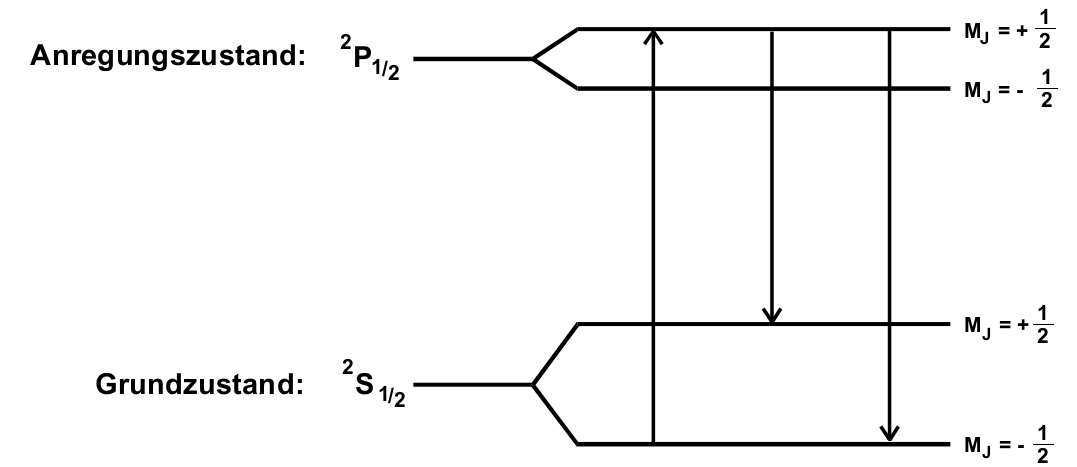
\includegraphics[height = 5cm]{pics/Uebergaenge_AlkaliAtom.png}
  \caption{Übergänge in einem Alkali-Atom.}
  \label{fig:AlkiBsp}
\end{figure}
\begin{figure}
  \centering
  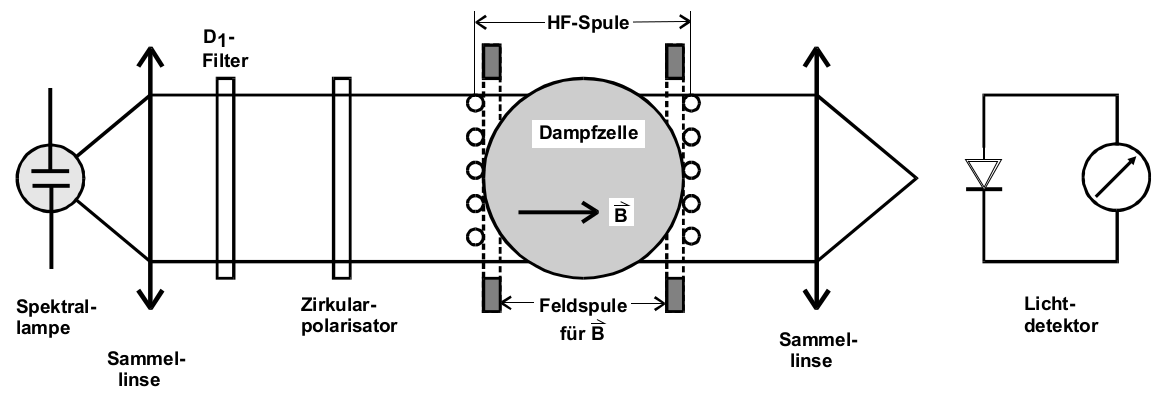
\includegraphics[height = 5cm]{pics/PrinzipiellerAufbau.png}
  \caption{Prinzipieller Aufbau.}
  \label{fig:BspAufbau}
\end{figure}
Nun wird das Verhalten der Transparenz der Dampfzelle bei anlegen eines Magnetfeldes 
diskutiert. Bei einem Magnetfeld um das Nullfeld kann nicht optisch gepumpt werden und somit 
bietet dies eine Möglichkeit das Erdmagnetfeld zu messen und zu kompensieren. Wird ein 
frequenzvariables Hochfrequenzfeld (RF) angelegt. Kann ein Pumpvorgang erzeugt werden der ein 
Inversion herbeiführt. Wird die Inversion herbeigeführt wird die Transparenz maximal. 
Erreicht das Magnetfeld den Wert 
\begin{equation}
\symup{h} \nu = g_J \mu_B B_m \Delta M_J  \iff
B_m = \frac{4\pi m_0}{\symup{e} g_J} \nu
\label{eq:Bm}
\end{equation}
tritt die induzierte Emission ein und die Transparenz der Dampfzelle nimmt ab. Beide Fälle sind 
in der Theoriekurve \ref{fig:TheoK} dargestellt.
\begin{figure}
  \centering
  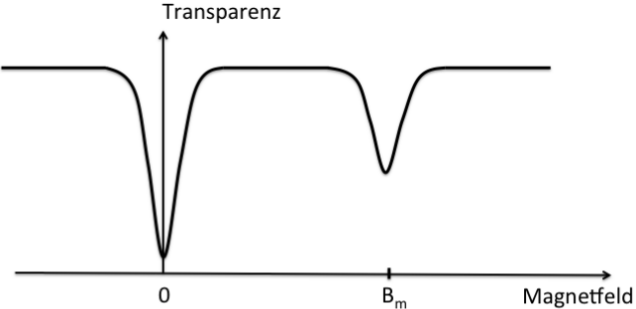
\includegraphics[height = 5cm]{pics/TheorieKurve.png}
  \caption{Theoriekurve der Transparenz der Dampfzelle in Abhängigkeit des Magnetfeldes.}
  \label{fig:TheoK}
\end{figure}
\FloatBarrier
\subsection{Der Quadratische Zeeman-Effekt}
Wird das B-Feld weiter erhöht müssen höhere Terme in \eqref{eq:UHF} berücksichtigt werden. 
Die Übergangsenergie verändert sich dann wie folgt:
\begin{equation}
U_{HF} = g_F \mu_B B +	g^{2}_F \mu^{2}_B B^2 \frac{1-2M_F}{\Delta E_{Hy}} - ... \; .
\label{eq:quadZ}
\end{equation}
Dabei bezeichnet $\Delta E_{Hy}$ die Hyperfeinstrukturaufspaltungen zwischen den Niveaus 
$F$ und $F+1$. Die Energie hängt nun von $M_F$ ab und wird daher als Quadratische Zeeman-Effekt 
bezeichnet. Ist ein Magnetfeld genügend groß weisen die Zeeman-Niveaus unterschiedliche 
Energien auf.  
\subsection{Transiente Effekte} 
An dieser Stelle wird das Verhalten des gepumpten Systems untersucht, während das 
RF schnell aus- und eingeschaltet wird.  Dabei soll das Magnetfeld als auch die 
RF-Frequenz auf eine Resonanz eingestellt sein. Resonanz bezeichnet hier den Punkt an dem 
die induzierte Emission eintritt. Im Resonanzfall ist das effektive B-Feld gleich dem RF-Feld. 
Daraus ergibt sich, dass der Spin $\vec{F}$ im rotierten Koordinatensystem mit der 
Lamor-Frequenz um $\vec{B}_{RF} = \vec{B}_{eff}$ präzediert. Die Lamor-Frequenz ist hierbei 
durch $\nu = \gamma B_{RF}$ gegeben. Daraus folgt eine Periode $T = \frac{1}{\gamma B_{RF}}$. 
Folglich lässt sich zwischen den Isotopen, die hier untersucht werden, die Relation 
>>>>>>>  Optisches Pumpen theo und Durch noch mal durchgeguckt
\begin{equation}
\frac{T_{87}}{T_{85}}=\frac{\gamma_{85}}{\gamma_{87}}
\label{eq:RelIso}
\end{equation}
für resonante RF-Felder bestimmen. Hierbei bezeichnet $\gamma$ das gyromagnetische Verhältnis
$\gamma = g_F \sfrac{\mu_0}{\symup{h}}$.
